\documentclass[12pt]{article}
\usepackage[margin=1.0in]{geometry}
\usepackage{amsmath}
\usepackage{listings}
\usepackage{graphicx}


\lstset{
    frame=tb, % draw a frame at the top and bottom of the code block
    tabsize=4, % tab space width
    showstringspaces=false, % don't mark spaces in strings
    numbers=left, % display line numbers on the left
    commentstyle=\color{green}, % comment color
    keywordstyle=\color{blue}, % keyword color
    stringstyle=\color{red} % string color
}





\title{Basic Roomba}
\author{Adithya Shastry}
\date{\today \\ CS342:Project 3}
\begin{document}
\maketitle
\newpage
\section{Overview}
The goal of this project was to make a small car that will avoid obstacles by turning. The car will take in sensory input(through the distance sensor), will have one button to turn the car on, and one to switch on a light on the car. This satisfies all of the criteria for the project. This project will incorporate ADCs, interrupts and GPIO in order to correctly work. I designed this project because I think it will be really cool to pull off something like this.


Note about the video: I decided to not include the tires in the video since I could not find anything to place my car on top of. It is possible to hear the motors if viewing them turn is difficult.


\section{Part Requirements}

\begin{table}[h!]
\centering
\begin{tabular}{|l|l|}
\hline
Part & Number \\ \hline
Wheels & 2 \\ \hline
Motors & 2 \\ \hline
ATmega Board & 1 \\ \hline
Computer & 1 \\ \hline
Distance Sensor & 1 \\ \hline
Switch & 1 \\ \hline
Button & 1 \\ \hline
Wires & Copious amounts \\ \hline
Battery Pack with batteries & 1 \\ \hline
Tape & Copious Amounts \\ \hline
Frame for Car & 1 \\ \hline
Twist Tie & 2 \\ \hline
\end{tabular}
\end{table}


\section{Circuit Implementation}
\newpage
\begin{figure}[h!]
\centering
\label{HardReq}
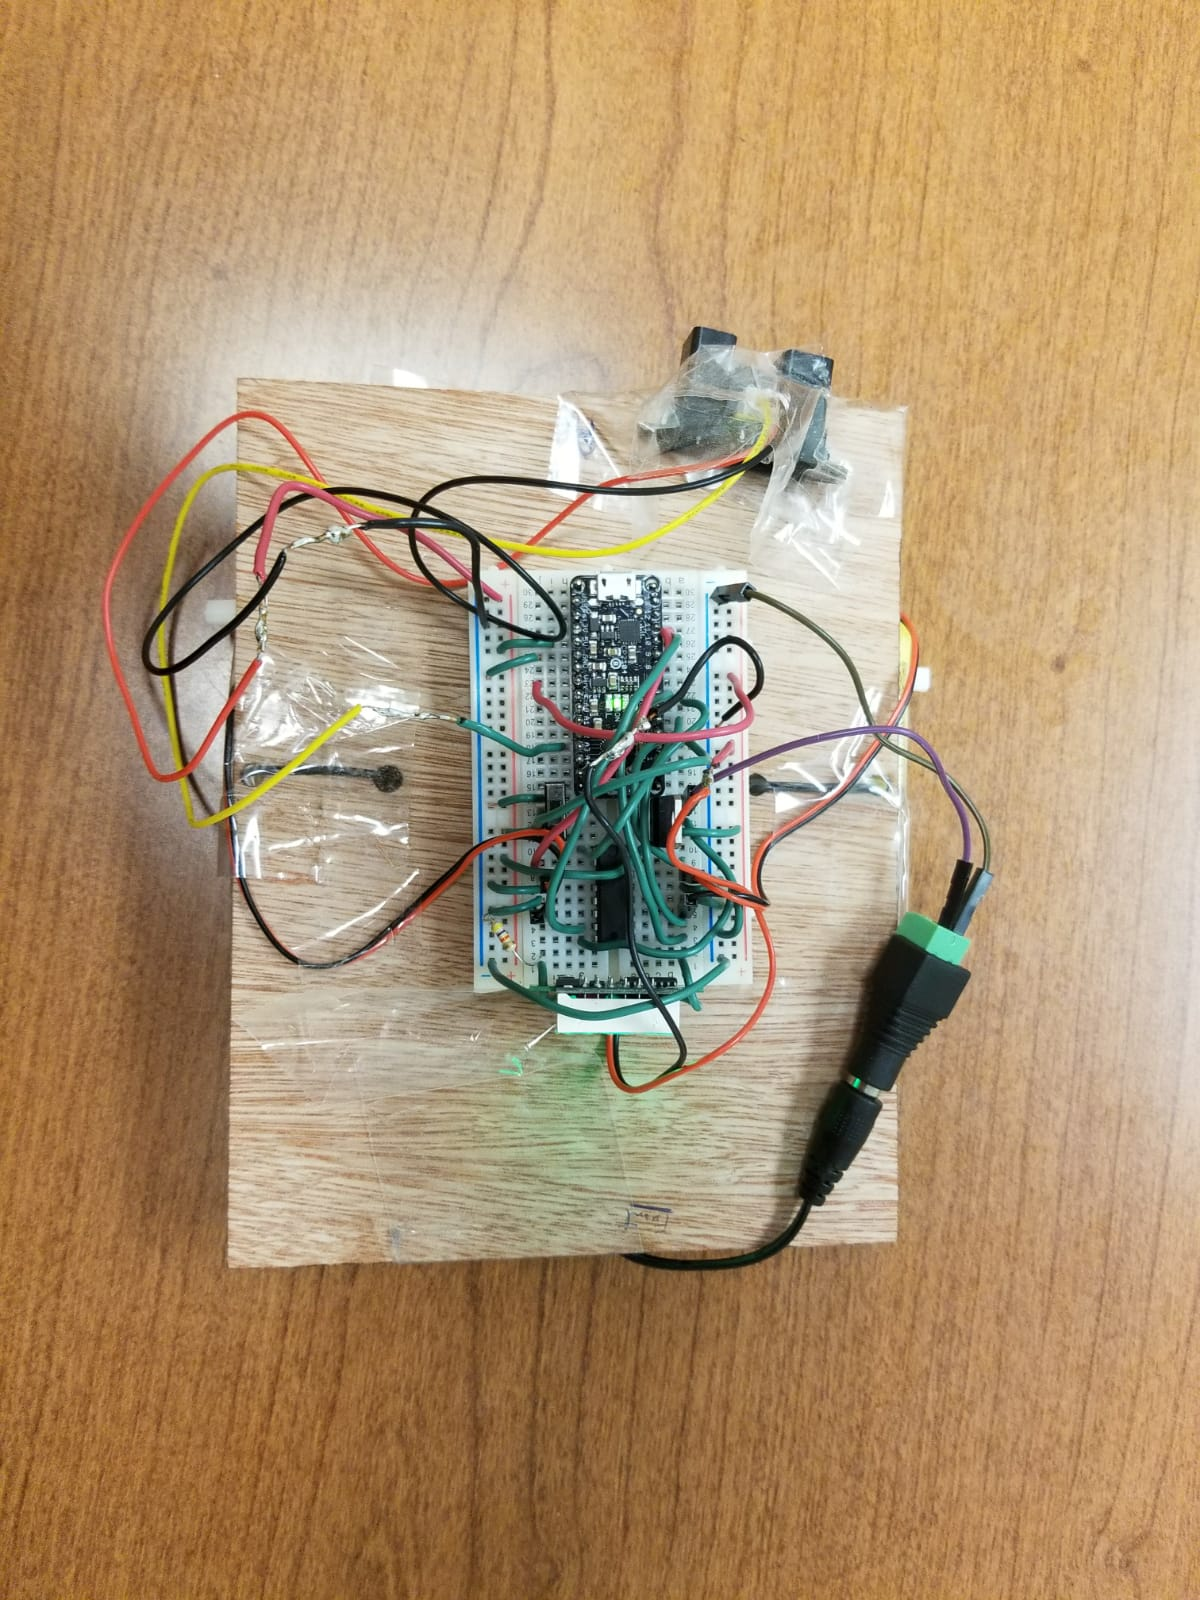
\includegraphics[scale=0.2]{image.jpeg}
\caption{Hardware Implementation}
\end{figure}


\section{Coding Implementation}


\begin{lstlisting}
#include <avr/io.h> // contains uint8_t and register 
//definitions
#include "USART.h"


uint16_t sensedADC=0; 
float mean=0.0;
int count=0;
 char msg[300];

//Enable the External Interrupt
  //Here you need to enable the motor interrupt and the 
  //ADC
ISR(INT0_vect){
  //Enable everything
  if(PINB & 0b00000100){
   //Enable GPIO 
  //For the Switch and Motor 2
  //WE will se the motor to go from 3 to 4 and 1 to 2 
  DDRD    = 0b01011000;
 
//  motor 1

DDRB    = 0b00011000;

  PORTB   =   0b00010000;
  PORTD    =  0b01001000;

  }
  else if(PINB&0b00000000){
    printString("Entered Else if");
  DDRB   =   0;
  DDRD    =  0;
 TIMSK1=0b00000100;//Enable COMP1A and COMP1B
 
}
}




ISR(ADC_vect){
//the ADC ISR
   //This will have logic for the actual conversion and 
   //the sliding window
    int N=200;

  
  sensedADC=ADCL;
  sensedADC|=(ADCH &0x03<<8);
  mean=mean *float(N-1)/float(N)+float(sensedADC)/float(N);

 

  
  //Convert the Mean to a distance in cm
  int distance= 0.0017*pow(mean,2)-1.0519*mean+197.75;

  sprintf(msg, "online mean: \t%d\n",int(distance));
  printString(msg);
  
   //Have logic for how to handle possible collisions 
   //with distances less than 20cm
    //Turn on the timer interrupt 1
    //Switch the direction of the motors

//I found that the equation I derrived from the data 
//collected from my sensor was not accurate, thus I 
//updated
//The equation to better fit the error in my equation
    
  if(distance<=150){
    printString("Distance Less than 65\n");
    TIMSK1=0;//Enable COMP1A and COMP1B
      PORTB   =   0;
  PORTD    =   0;
    ADMUX=0;
  }
    
}







ISR(TIMER1_COMPB_vect){
  
}



int main(){

  initUSART();  
    



 //ADC 
 //The sensor is connected to A3
  DDRC    = 0b00000000;
  PORTC   = 0b00000000;


  
  

   TCCR0A  = 0b11000011;
  TCCR0B  = 0b00000100;
  OCR0A   = 10;



  //Enable Timer 1 COMPA for turning duration
  //COMPB for The ADC
  //We can have this count to 1ms and use a counter to 
  //count the correct duration. This will make testing easier

  TCCR1A=0b00000000;
  TCCR1B=0b00001011;//Set to CTC mode and have prescale of 64
  OCR1AL=250;
  OCR1BL=250;//Want to be able to use COMP1B
  TIMSK1=0b00000100;//Enable COMP1A and COMP1B



  //Enable ADC control
 ADMUX=0b01000011;
 ADCSRA=0b11101111;
 ADCSRB=0b00000101;//Set the ADC to run based on Compare match B


  //Enable the Switch with Pin change Interrupt
  //PCINT18---->PCI2-------->PD2

  //Use EINT0
  EICRA= 0b00001101;//Falling edge for Eint1 and any 
  //logical change for EINT0
  EIMSK= 0b00000011;
  

  
  



  



  //Enable Global Interrupts
  SREG|=0x80;

  while(true){}
}
\end{lstlisting}

\section{Testing and Possible Further Improvements}
Further imporvements would include using better motors to allow the car to be fully mobile, even with the added weight of the battery pack. During my testing for this, I found that the normal force on the wheels of the car, were too large for the motors to actually move the car.Therefore, I had to remove the battery pack from the car. A stronger motor, one with greater torque, would greatly help carry the added weight of the battery pack.

\section{Conclusion}
Overall,this was a great project to work on because it taught me not only how to set up the software, but also how to set up the physical parts of the car in order for it to actually work. In order to do this I had to utilize a lot of the physics I had learned freshman year. This is was a really cool experience for me because I never had to really apply things learned in physics like that before!
\end{document}